\section{Cartier's big Witt functor}
Until recently, constructing Witt vectors was an arduous task. Using Lenstra's construction, it will become a (rather long) walk in the park. In this second installment, Witt's motivation for introducing these objects is given, and a general strategy is outlined.

\subsection{Motivation}
For a field~$K$ containing a primitive~$m$-th root of unity, Kummer theory says that every extension~$K(\sqrt[m]a)/K$ is cyclic of degree~$d\divides m$, and conversely, every cyclic extension of degree~$m$ is obtained that way. This basically means adjoining the root of a polynomial~$X^{m}-a$. Using these results, you can set up very nice Galois-like correspondences, but the catch is that the characteristic of~$K$ cannot divide~$m$. To remedy part of this, Artin and Schreier came up with a theory where~$m = \operatorname{char}(K) = p$. By using polynomials of the form~$X^{p}-X-a$, they were able to prove statements rather analogous to the above. The next step would be to look at fields of characteristic~$p$, with extensions of degree~$p^{n}$. This turned out to be rather difficult, but Abraham Albert managed to solve the problem in the thirties by means of some very technical constructions.

Enter our hero, Witt, who introduced the ring~$\mathrm{W}_{m}(K)$ of~$p$-typical Witt vectors of length~$m$. By constructing an (additive) group endomorphism~$\wp\colon\mathrm{W}_{m}(K)\to\mathrm{W}_{m}(K)$, he proved that every such extension could be written as~$K(\wp^{−1}(D))$ for some order~$p^{m}$ cyclic subgroup~$D\subset\mathrm{W}_{m}(K)/\wp(\mathrm{W}_{m}(K))$, and conversely. For a more detailed account of this process, and for some more applications of the~$p$-typical vectors, check out Harder's (translated) article An Essay on Witt Vectors to be found in~\cite{witt-collected}.

\subsection{Modus operandi}
\begin{wrapfigure}{r}{.35\textwidth}
  \centering
  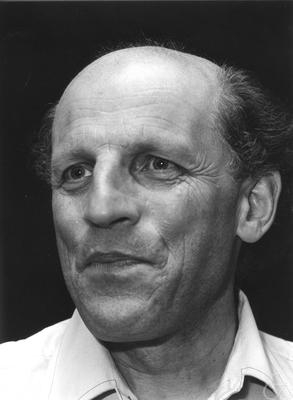
\includegraphics[width=.3\textwidth]{playing-witt-rings/cartier}
  \caption{Pierre Cartier}
\end{wrapfigure}
Instead of constructing Witt's~$p$-typical vectors from scratch, most of the literature describes an endofunctor in the category of commutative rings with unity, mapping a ring~$A$ into the ring of big Witt vectors~$\mathrm{W}(A)$. Contrary to popular belief, this approach wasn't worked out by Witt, but by Pierre Cartier in his 1967 paper~\cite{cartier}. The original (small) Witt vectors can then be found by applying this functor to~$\mathbb{F}_{p^{n}}$, but the universal construction has turned out to be immensely important in modern algebra and arithmetic algebraic geometry. Lenstra's construction is not the standard one found in the literature, but is a lot easier. For every commutative, unital ring~$A$, we'll end up with a ring~$\Lambda(A)$ which is isomorphic to~$\mathrm{W}(A)$.

\subsection{Battle plans}
Because there are lots of structures involved, I've added a table at the end of this post which might come in handy while reading the series (notice that the superscript~$^{*}$ is used to indicate the unit group). Ok, let's get to it. For a commutative, unital ring~$A$, identify~$\Lambda(A)$ as a set with~$1+TA[\![T]\!]$. The multiplication of power series, denoted by~$\times$, turns this set into an abelian group. This way,~$\Lambda(A)$ corresponds to the kernel of~$\operatorname{pr}_{0}^{*}$, which is the morphism of unit groups induced by projecting an invertible power series on its constant factor. The goal is to put a nice ring structure on~$\Lambda(A)$ which turns~$\Lambda$ into a functor and has~$\times$ as its addition. This will be very hard to do directly, and we'll proceed in a couple of steps.

\subsection{Discretion advised}
To start, we'll define a discrete analogue of~$\Lambda(A)$, denoted~$\Lambda_{n}(A)$. The idea is to repeat the process given above for~$A[T]/(T^{n+1})$, the algebra of truncated polynomials. If we define~$\operatorname{pr}_{n}^{0}$ as projection on the constant factor, this will induce a group morphism on the unit groups, and~$\Lambda_{n}(A)$ is defined as the kernel of~$(\operatorname{pr}_{n}^{0})^{*}$. Taking the projective limit, we recover~$\Lambda(A)$. If we manage to put a ring structure on~$\Lambda_{n}(A)$, it might be possible to extend this to~$\Lambda(A)$, provided we have nice functorial properties.

\subsection{Digging deeper}

Define~$\mathrm{M}_{n}(A)$ as the subgroup of~$\Lambda_{n}(A)$, generated by elements of the form~$1-aT$, for~$a \in A$. It's easy to check that these elements are invertible in~$A[T]/(T^{n+1})$, so the definition is sound. This abelian group can be made into a commutative ring with new multiplication~$\ast$, satisfying the following property:
\begin{equation}
  \label{equation:multiplication}
  (1-aT)^{-1} \ast (1-bT)^{-1} = (1-abT)^{-1}, a,b \in A.
\end{equation}
If we are able to lift this structure to~$\Lambda_{n}(A)$, we just might have our Witt ring! But first, how to define a nice multiplication on~$\mathrm{M}_{n}(A)$?

For every~$a \in A$, there's an~$A$-endomorphism of~$A[T]/(T^{n+1})$ which sends~$T$ to~$aT$. This induces an endomorphism of the unit group, and thus of~$\Lambda_{n}(A)$, which we'll denote by~$\phi_{n}^{a}$. Now look at the additive subgroup of~$\operatorname{End}(\Lambda_{n}(A))$ generated by all the~$\phi_{n}^{a}$. From the definition of these functions, it's clear that~$\phi_{n}^{a} \circ \phi_{n}^{b}=\phi_{n}^{ab}$, and the subgroup becomes a commutative subring free of charge. Denote this ring by~$E$. It acts naturally on~$\Lambda_{n}(A)$, turning it into an~$E$-module. For notational convenience, we'll write this action exponentially.

Look at the following~$E$-module morphism, where~$E$ has the regular~$E$-module structure:
\begin{equation}
  m\colon E \to \Lambda_{n}(A): \ \phi_{n}^{a} \mapsto (1-T)^{-\phi_{n}^{a}}. 
\end{equation}
Rewriting the image we get
\begin{equation}
  (1-T)^{-\phi_{n}^{a}}= \phi_{n}^{a} \cdot (1-T)^{-1} =(1-aT)^{-1}. 
\end{equation}
Since this is in particular a group morphism, and the generators of~$E$ get mapped to the generators of the group~$\mathrm{M}_{n}(A)$, the image is equal to~$\mathrm{M}_{n}(A)$. The kernel of~$m$ is a two-sided ideal of~$E$, and we get a group isomorphism:
\begin{equation}
  E/I \cong \mathrm{M}_{n}(A). 
\end{equation}
Since the quotient on the left-hand side is also well defined within ring theory,~$E/I$ becomes a ring. Using transport of structure, we can make~$\mathrm{M}_{n}(A)$ into a ring. In this ring, \eqref{equation:multiplication} obviously holds, and~$(1-T)^{-1}$ is the multiplicative unit. You can check for yourself that this makes $\mathrm{M}_{n}$ into a functor and that the `projection' maps~$\mathrm{M}_{n+1} \to \mathrm{M}_{n}$ are natural transformations, which is very easy. In the next post, we'll try to elevate this structure to~$\Lambda_{n}(A)$.

\begin{table}[tp]
  \centering
  % as per http://texblog.net/latex-archive/layout/centering-figure-table/ 
  \noindent\makebox[\textwidth]{%
    \begin{tabular}{p{.2\textwidth}p{.31\textwidth}p{.5\textwidth}}
      \toprule
      \emph{Object} & \emph{Structure} & \emph{Operation} \\\midrule
      ${(A[\![T]\!],+,\times)}$ & algebra & sum and multiplication of power series \\
      ${(\Lambda(A),\times)}$ & subgroup of~${A[\![T]\!]^{*}}$ & multiplication of power series \\
      ${(\Lambda_{n}(A),\times)}$ & subgroup of ${A[T]/(T^{n+1})}$ & multiplication of polynomials \\
      ${(\mathrm{M}_{n}(A),\times)}$ & subgroup of ${\Lambda_{n}(A)}$ & multiplication of polynomials \\
      ${(\operatorname{End}(\Lambda_{n}(A)),\times,\circ)}$ & endomorphism ring & pointwise multiplication of polynomials and composition \\
      ${(E,\times,\circ)}$ & subring of ${\operatorname{End}(\Lambda_{n}(A))}$ & pointwise multiplication of polynomials and composition \\
      \bottomrule
    \end{tabular}
  }
  \caption{All structures involved}
  \label{table:witt-vector-objects-overview}
\end{table}
